\section{\tl{Raw data vs DCCA}}
\en{As mentioned before, we consider as the baseline results the SVM classification on the imaging and genetic data taken directly after LR on the ADNI dataset, and then compare them with the methods we experimented with. }
\subsection{\en{Without scaling or balancing:}}
\en{
\begin{figure}[H]
    \centering
    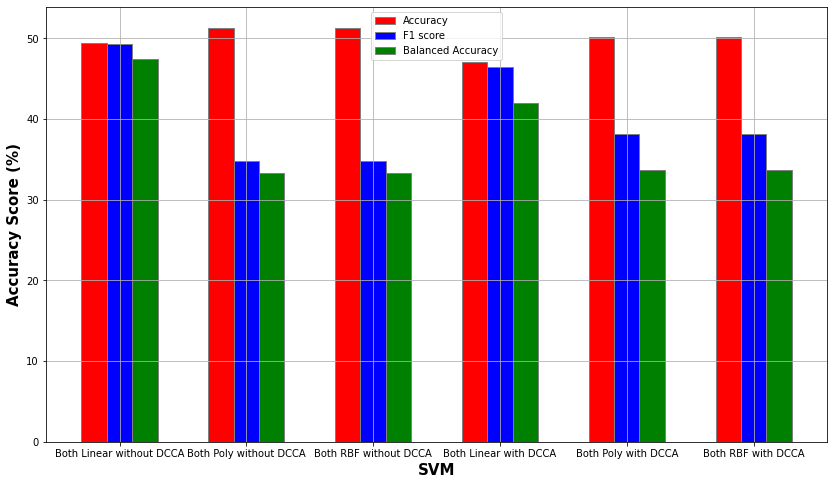
\includegraphics[width=\textwidth]{figures/Results/RAW/Raw_Both_out.png}
    \caption[\en{Classification metric scores using Both views on Raw vs DCCA data}]{\en{Classification metric scores using Both views (Imaging and Genetic), on the SVM kernels (Linear, Polynomial, RBF), using raw data (3 left bar groups) vs using DCCA (3 right bar groups)}}
\end{figure}

\begin{figure}[H]
    \centering
    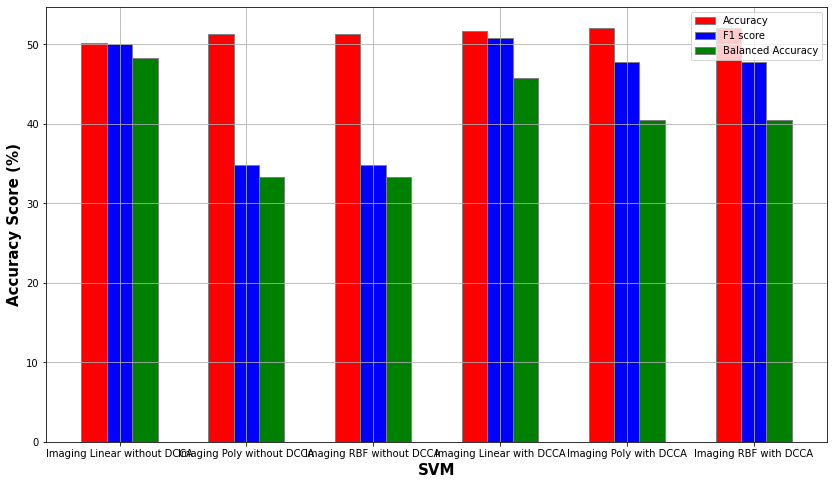
\includegraphics[width=\textwidth]{figures/Results/RAW/Raw_Ima_out.png}
    \caption[\en{Classification metric scores using Imaging view on Raw vs DCCA data}]{\en{Classification metric scores using only the Imaging view, on the SVM kernels (Linear, Polynomial, RBF), using raw data (3 left bar groups) vs using DCCA transformed imaging data, trained on both views (3 right bar groups)}}
\end{figure}

\begin{figure}[H]
    \centering
    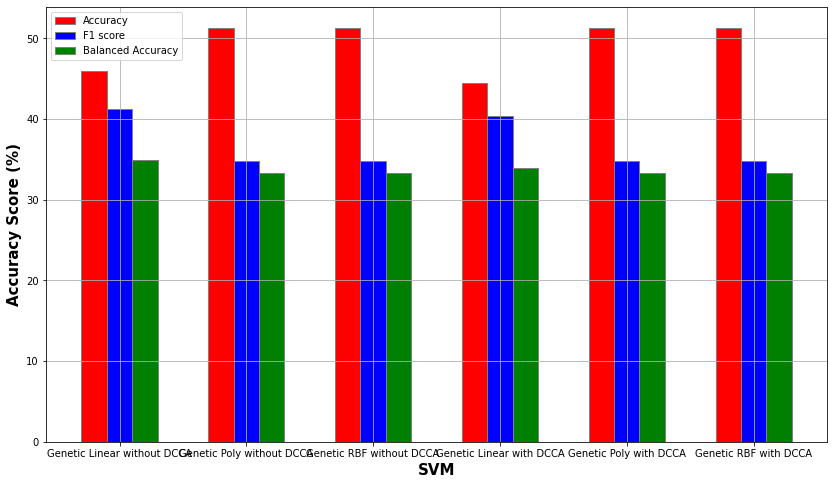
\includegraphics[width=\textwidth]{figures/Results/RAW/Raw_Gen_out.png}
    \caption[\en{Classification metric scores using Genetic view on Raw vs DCCA data}]{\en{Classification metric scores using only the Genetic view, on the SVM kernels (Linear, Polynomial, RBF), using raw data (3 left bar groups) vs using DCCA transformed genetic data, trained on both views (3 right bar groups)}}
\end{figure}

% \begin{figure}[H]
%     \centering
%     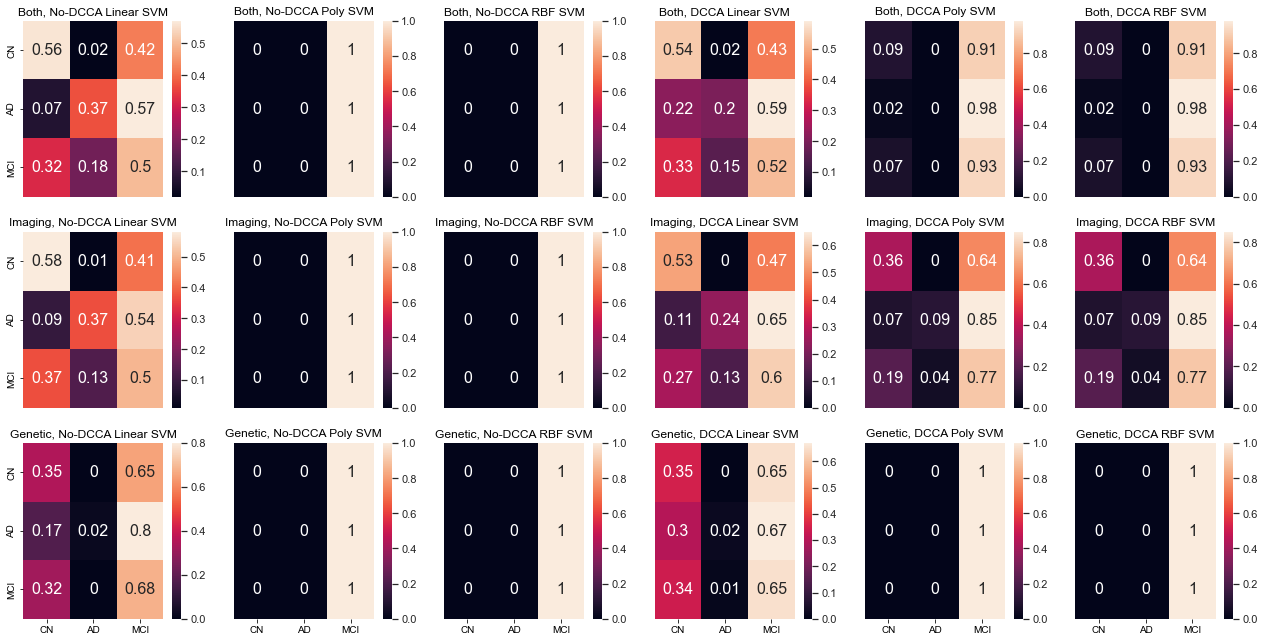
\includegraphics[width=\textwidth]{figures/Results/RAW/Raw_CM_out.png}
%     \caption[\en{Confusion Matrices of Raw vs DCCA data}]{\en{The Confusion Matrices for each class, per model, using both views (top row), only the imaging view (middle row), and only the genetic view (bottom row). The three left columns represent the CM of the raw data classification, while the three right columns represent the CM of the DCCA transformed data classification.}}
% \end{figure}

\begin{figure}[H]
    \centering
    \includegraphics[width=\textwidth]{figures/Results/RAW/Bagging_RAW_out.png}
    \caption[\en{Bagging Classification metrics}]{\en{Classification metric using Bagging on the imaging and genetic data.}}
\end{figure}

% \begin{figure}[H]
%     \centering
%     \includegraphics[width=\textwidth]{figures/Results/RAW/Bagging_RAW_CM_out.png}
%     \caption[\en{Bagging Confusion Matrices}]{\en{The Confusion Matrices for each class, with Bagging, for the imaging and genetic data.}}
% \end{figure}

\begin{figure}[H]
    \centering
    \includegraphics[width=\textwidth]{figures/Results/RAW/AdaBoost_RAW_out.png}
    \caption[\en{AdaBoost Classification metrics}]{\en{Classification metric using AdaBoost on the imaging and genetic data.}}
\end{figure}

% \begin{figure}[H]
%     \centering
%     \includegraphics[width=\textwidth]{figures/Results/RAW/AdaBoost_RAW_CM_out.png}
%     \caption[\en{AdaBoost Confusion Matrices}]{\en{The Confusion Matrices for each class, with AdaBoost, for the imaging and genetic data.}}
% \end{figure}

}
\subsection{\en{With scaling and balancing:}}
\en{
\begin{figure}[H]
    \centering
    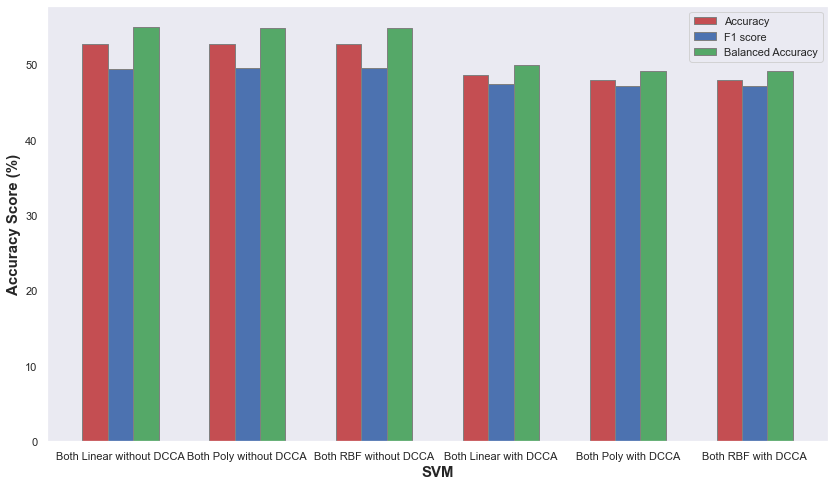
\includegraphics[width=\textwidth]{figures/Results/RAW/Raw_Both_with.png}
    \caption[\en{Classification metric scores using Both views on Raw vs DCCA data with scaling and balancing}]{\en{Classification metric scores using Both views (Imaging and Genetic), on the SVM kernels (Linear, Polynomial, RBF), using raw data (3 left bar groups) vs using DCCA (3 right bar groups)}}
\end{figure}

\begin{figure}[H]
    \centering
    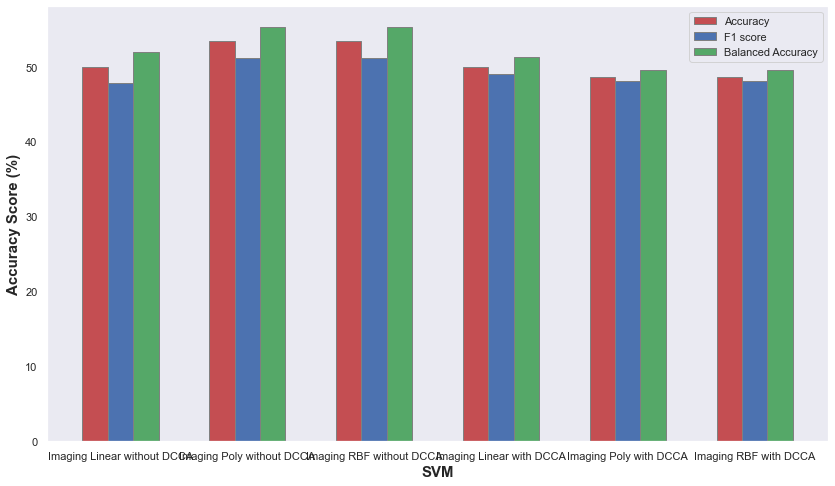
\includegraphics[width=\textwidth]{figures/Results/RAW/Raw_Ima_with.png}
    \caption[\en{Classification metric scores using Imaging view on Raw vs DCCA data with scaling and balancing}]{\en{Classification metric scores using only the Imaging view, on the SVM kernels (Linear, Polynomial, RBF), using raw data (3 left bar groups) vs using DCCA transformed imaging data, trained on both views (3 right bar groups)}}
\end{figure}

\begin{figure}[H]
    \centering
    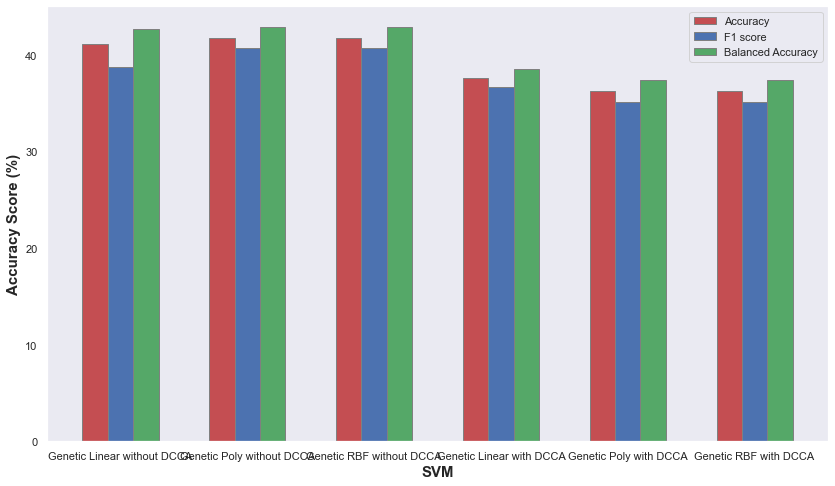
\includegraphics[width=\textwidth]{figures/Results/RAW/Raw_Gen_with.png}
    \caption[\en{Classification metric scores using Genetic view on Raw vs DCCA data with scaling and balancing}]{\en{Classification metric scores using only the Genetic view, on the SVM kernels (Linear, Polynomial, RBF), using raw data (3 left bar groups) vs using DCCA transformed genetic data, trained on both views (3 right bar groups)}}
\end{figure}

% \begin{figure}[H]
%     \centering
%     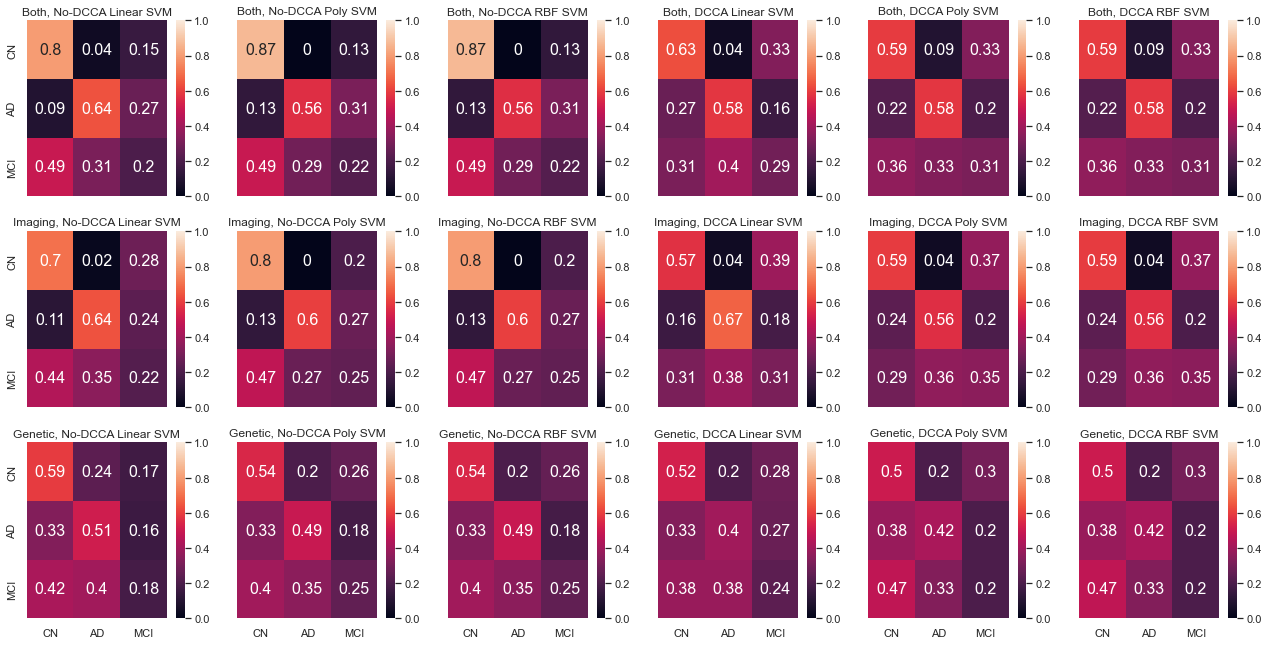
\includegraphics[width=\textwidth]{figures/Results/RAW/Raw_CM_with.png}
%     \caption[\en{Confusion Matrices of Raw vs DCCA data with scaling and balancing}]{\en{The Confusion Matrices for each class, per model, using both views (top row), only the imaging view (middle row), and only the genetic view (bottom row). The three left columns represent the CM of the raw data classification, while the three right columns represent the CM of the DCCA transformed data classification.}}
% \end{figure}

\begin{figure}[H]
    \centering
    \includegraphics[width=\textwidth]{figures/Results/RAW/Bagging_RAW_with.png}
    \caption[\en{Bagging Classification metrics with scaling and balancing}]{\en{Classification metric using Bagging on the imaging and genetic data.}}
\end{figure}

% \begin{figure}[H]
%     \centering
%     \includegraphics[width=\textwidth]{figures/Results/RAW/Bagging_RAW_CM_with.png}
%     \caption[\en{Bagging Confusion Matrices with scaling and balancing}]{\en{The Confusion Matrices for each class, with Bagging, for the imaging and genetic data.}}
% \end{figure}

\begin{figure}[H]
    \centering
    \includegraphics[width=\textwidth]{figures/Results/RAW/AdaBoost_RAW_with.png}
    \caption[\en{AdaBoost Classification metrics with scaling and balancing}]{\en{Classification metric using AdaBoost on the imaging and genetic data.}}
\end{figure}

% \begin{figure}[H]
%     \centering
%     \includegraphics[width=\textwidth]{figures/Results/RAW/AdaBoost_RAW_CM_with.png}
%     \caption[\en{AdaBoost Confusion Matrices with scaling and balancing}]{\en{The Confusion Matrices for each class, with AdaBoost, for the imaging and genetic data.}}
% \end{figure}

The following tables present the complete results for the raw data, as well as the DCCA transformed data, for each model, for each metric, for each view, and either with or without scaling and balancing. With green are highlighted the best values for each metric, depending on whether scaling and balancing were applied:

\begin{figure} [H]
    \centering
    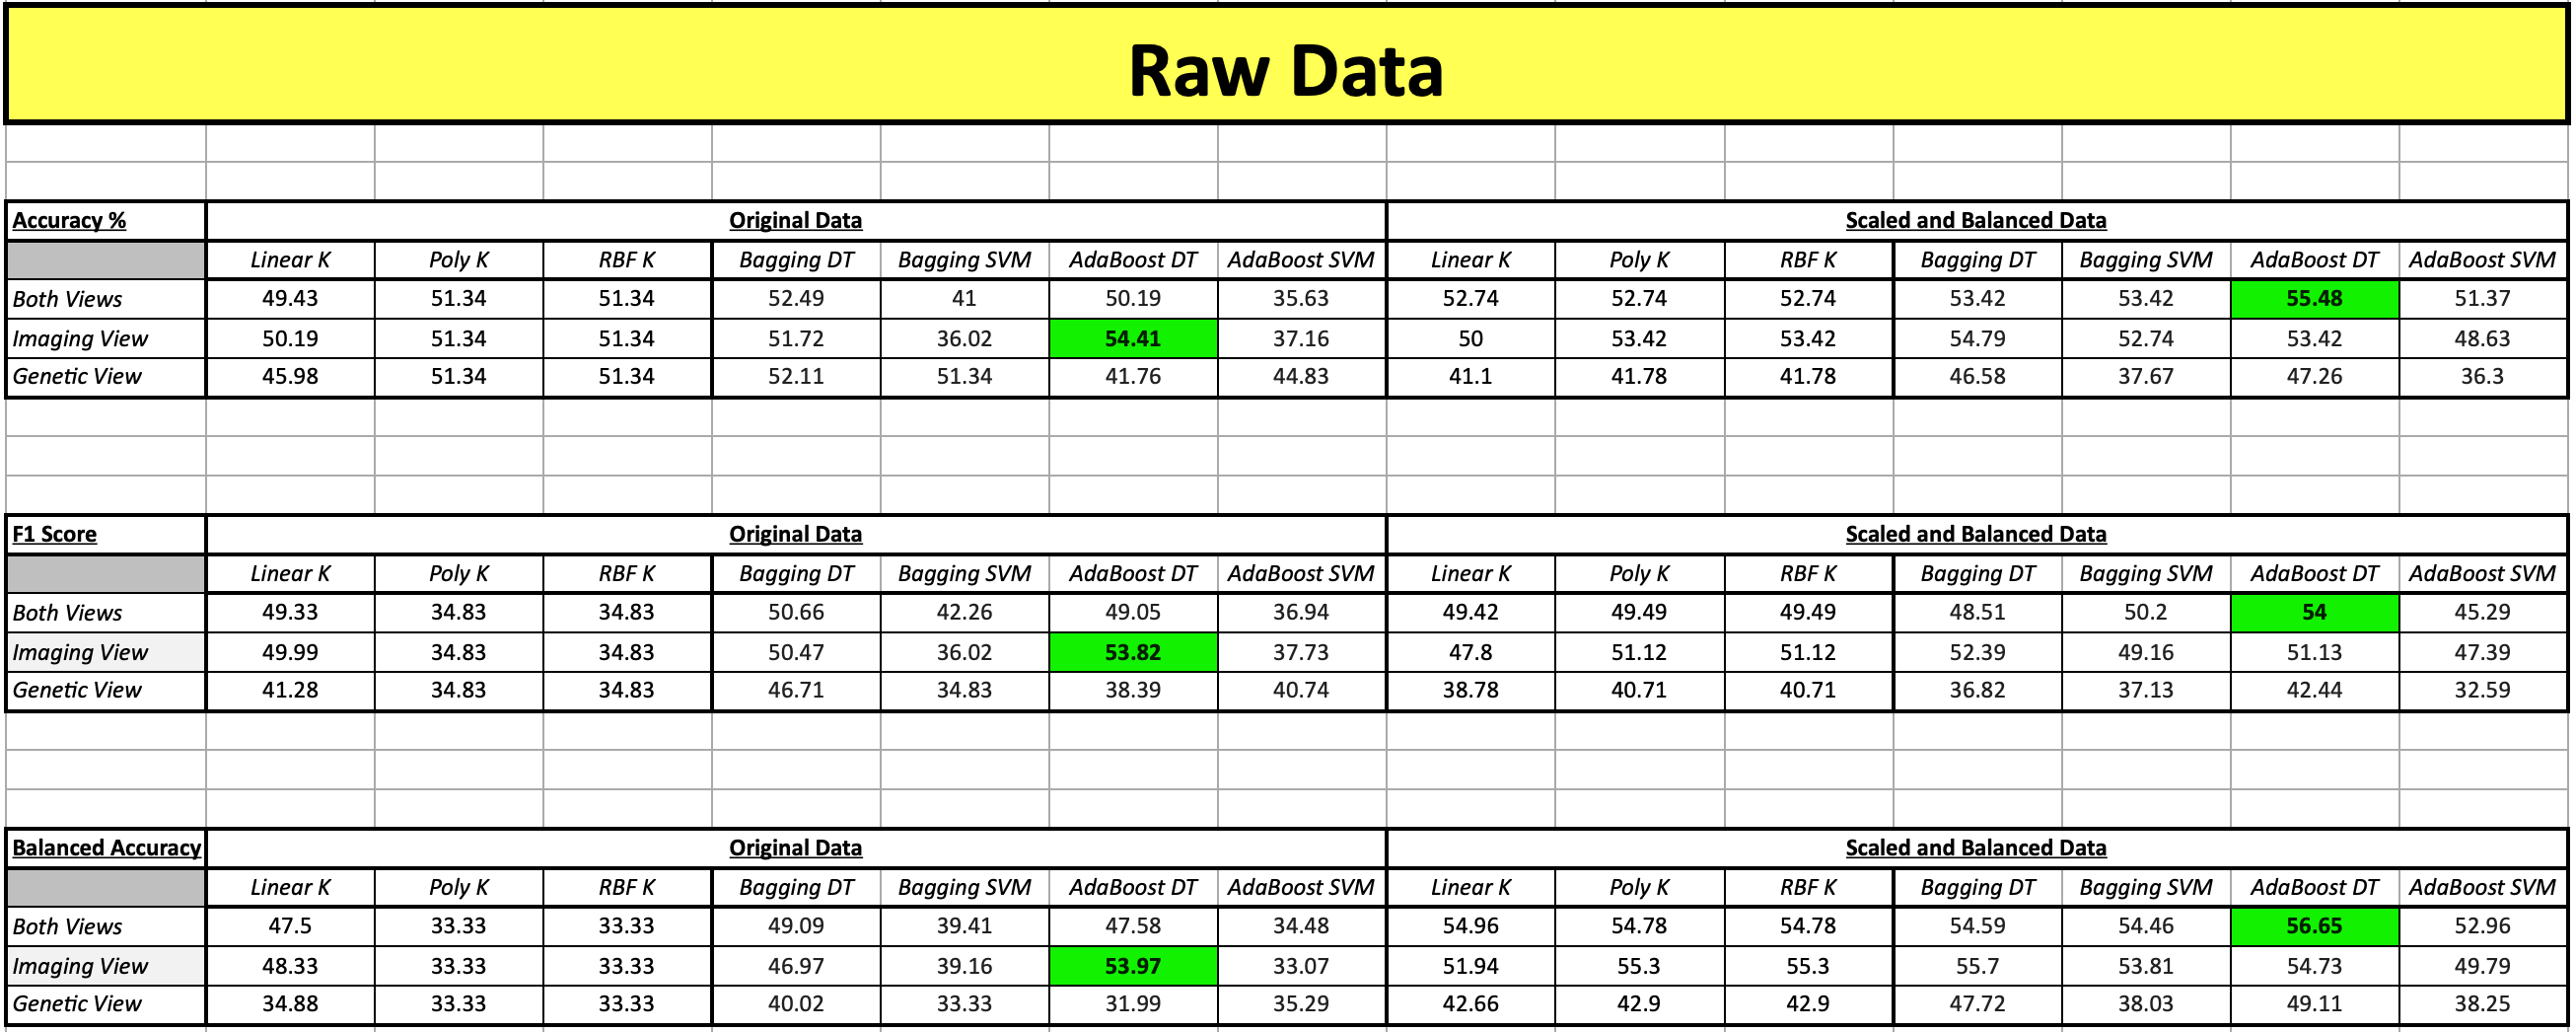
\includegraphics[width=\textwidth]{figures/Results/Analytical_Table_Raw.png}
    \caption[\en{Analytical table of results for raw data classification}]{\en{For each model and classifier, the metric scores for raw data classification are presented. Highlighted green are the best performing models, for each metric.}}
    \label{fig: Summary Table for classification scores for raw data}
\end{figure}

\begin{figure} [H]
    \centering
    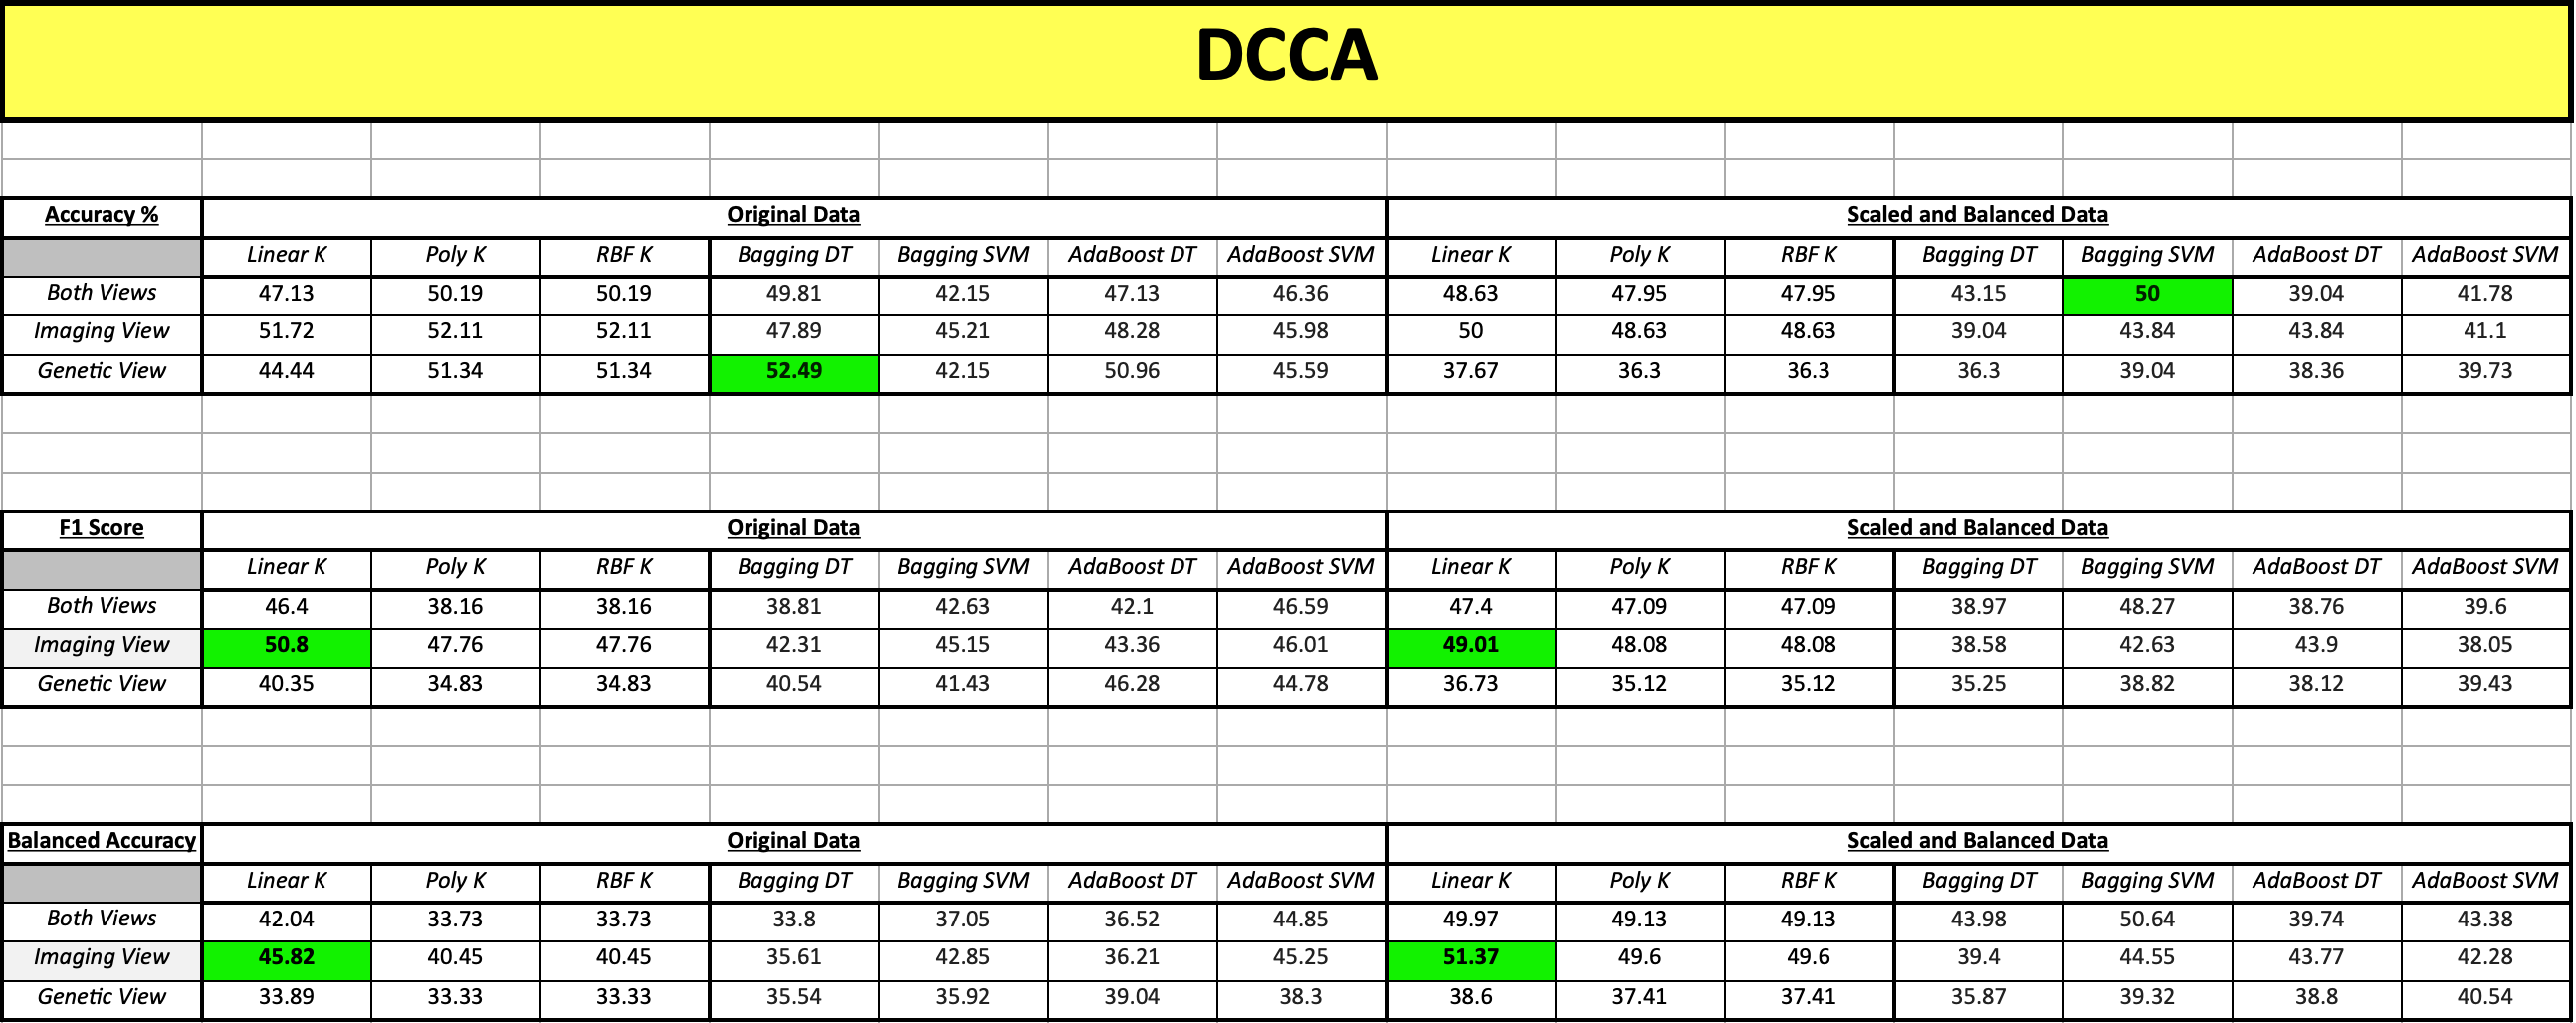
\includegraphics[width=\textwidth]{figures/Results/Analytical_Table_DCCA.png}
    \caption[\en{Analytical table of results for DCCA transformed data classification}]{\en{For each model and classifier, the metric scores for DCCA transformed data classification are presented. Highlighted green are the best performing models, for each metric.}}
    \label{fig: Summary Table for classification scores for DCCA data}
\end{figure}

}